\section{Introduction}

Large Language Models (LLMs) have become foundational infrastructure for modern service operations, powering customer-facing chatbots \citep{anthropic2023claude, bai2023qwen, openai2024gpt4technicalreport, deepseekai2025deepseekr1incentivizingreasoningcapability}, intelligent search engines \citep{google2023bard, microsoft2023bing}, and programming assistants \citep{copilot, claude_3_7}. As these systems transition from experimental deployments to mission-critical services handling millions of concurrent users, efficient resource management has emerged as a defining challenge for sustainable operations \citep{devlin2019bert, brown2020language, kaplan2020scaling, ouyang2022training, wei2022emergent, wei2022chain, touvron2023llama}. The computational bottleneck lies in \textit{inference}---the process of generating responses to user queries in real-time---which requires sophisticated scheduling to balance service quality (response latency) against operational efficiency (throughput and resource utilization) \citep{garcia2019estimation}.

The operational imperatives are substantial. Systems like ChatGPT incur daily inference costs exceeding \$700,000, with significant carbon emissions from high electricity usage \citep{patel2023peeling, patterson2021carbon}. Beyond direct costs, inefficient resource allocation creates service quality problems: excessive latency frustrates users and reduces engagement, while underutilized resources represent wasted capacity \citep{strubell2019energy, desislavov2021compute}. Effective scheduling strategies can simultaneously reduce costs, improve service responsiveness, and enhance sustainability \citep{wu2022sustainable}---making this a quintessential operations management challenge at the intersection of technology and service delivery.

Unlike traditional service systems where resource requirements are static and known at arrival, LLM inference presents unique operational complexities. To understand the scheduling challenge, consider the resource allocation dynamics during LLM inference. Figure~\ref{fig:intro_example} illustrates how a single user query---such as ``Is apple a fruit?''---transforms into a multi-stage resource management problem. The inference pipeline operates in two distinct phases that create fundamentally different demands on the system:
\begin{itemize}
    \item \textbf{Prefill Phase (stage 0)}: Upon receiving the prompt, the model first tokenizes the input into a sequence of discrete units (e.g., ``Is'', ``apple'', ``a'', ``fruit'', ``?''). These tokens are then embedded and simultaneously processed in a single forward pass to compute the \textit{Key-Value (KV) cache}, which stores intermediate representations (i.e., attention keys and values) for each token. These precomputed values are critical for enabling efficient reuse during subsequent decoding steps. This phase corresponds to Stage 0 in Figure~\ref{fig:intro_example}, where all prompt tokens are embedded and their KV representations are added to the cache.

    \item \textbf{Decode Phase (stages 1 to $l^\prime$)}: After the prefill phase, the model enters the decode phase, where it generates the output one token at a time. At each stage, the model queries the existing KV cache to compute the next token, appends the new token to the output sequence, and updates the KV cache with its key-value pair. For instance, the model might first generate ``Yes'' (Stage 1), then ``it'' (Stage 2), followed by ``is'' (Stage 3), and finally the ``End of Sequence'' (EOS) token (Stage 4). This progression is depicted in the lower part of Figure~\ref{fig:intro_example}. Each token generation step involves both reading from and writing to the KV cache, resulting in a memory footprint that grows linearly with the length of the generated sequence.
\end{itemize}

\begin{figure}
    \centering
    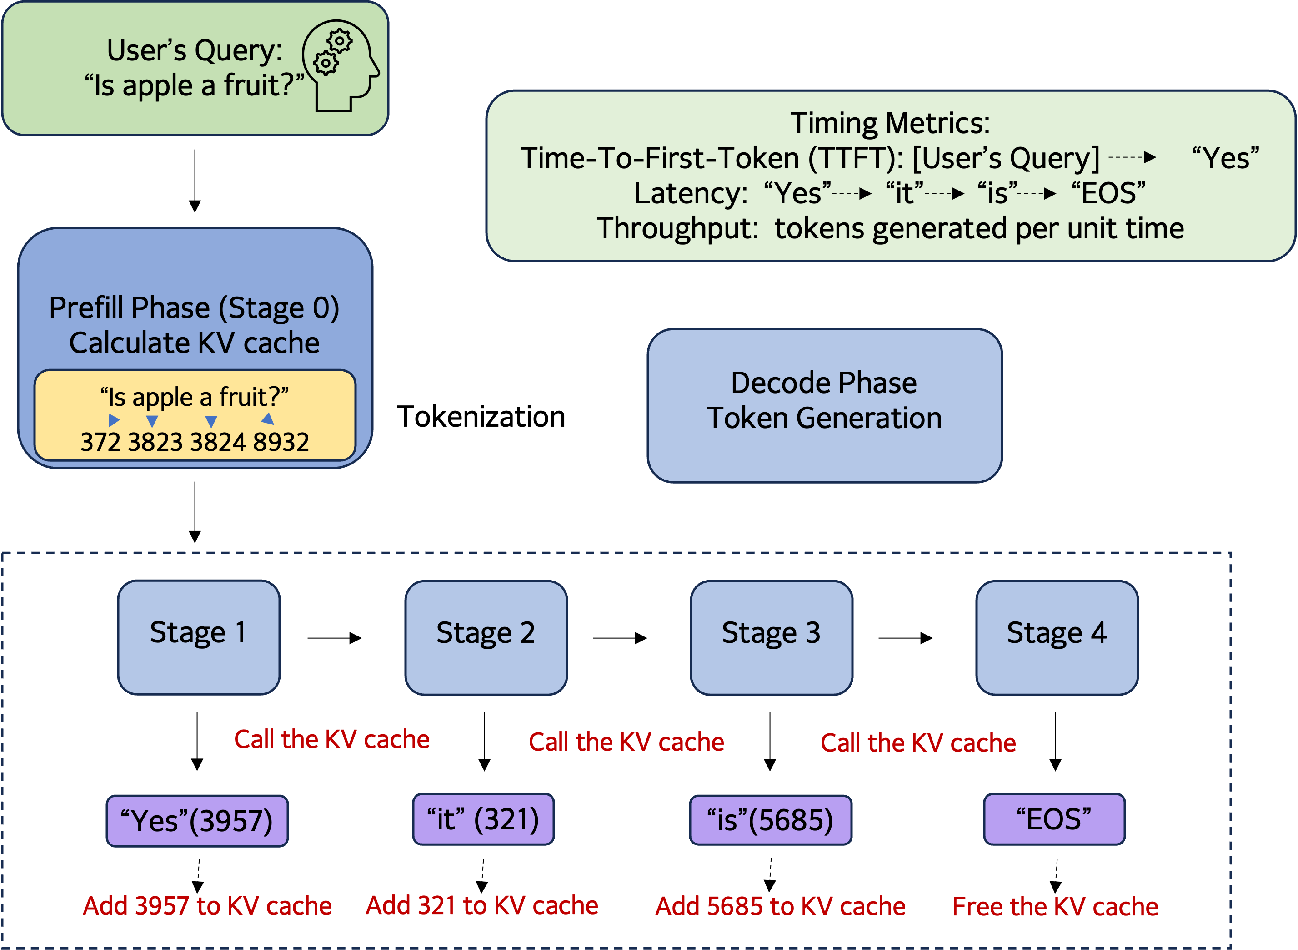
\includegraphics[width=0.6\linewidth]{Experiments_pdf/fig_intro.pdf}
    \caption{An example of LLM inference.}
    \label{fig:intro_example}
\end{figure}

Figure~\ref{fig:intro_example} also highlights key performance metrics in LLM inference:
\begin{itemize}
    \item \textbf{Time-To-First-Token (TTFT)} measures the latency from user input to the first generated token.
    \item \textbf{Latency} refers to the total time required to complete the generation of all output tokens.
    \item \textbf{Throughput} captures the average number of tokens generated per unit time.
\end{itemize}

From an operations perspective, this two-phase structure with unpredictable memory growth creates a novel scheduling problem that differs fundamentally from classical job shop or queueing models. The challenge resembles revenue management under capacity constraints, but with dynamic ``capacity consumption'' (KV cache size) that grows during service delivery and becomes fully known only after commitment---a characteristic absent from airline or hotel settings. The KV cache is essential for computational efficiency, as it prevents the model from recalculating the attention history for each new token. Without it, the computational cost would scale quadratically with the sequence length, making real-time inference infeasible. However, the expanding KV cache poses a significant resource allocation challenge, as the memory footprint grows unpredictably during the decode phase. This variability, combined with stochastic prompt arrivals and differing response lengths, complicates resource allocation on hardware with finite capacity, such as GPUs. Exceeding memory limits can force the system to offload data to slower storage mediums, degrading performance and increasing latency \citep{tay2022efficient, kang2024gear, hooper2025kvquant}.

\paragraph{Why Traditional Operations Research Approaches Fail.}
Scheduling LLM inference tasks involves grouping prompts into \textit{batches} processed concurrently on a GPU, combining prefill and decode phases to optimize resource use. This process is constrained by GPU memory limits, as the KV cache grows with each generated token, restricting the number of active prompts. Traditional scheduling methods, such as Shortest Job First (SJF)---a classic policy that minimizes mean completion time in conventional queueing systems \citep{conway1967theory}---prove inadequate because they assume fixed job sizes and known processing times. 

Consider a concrete example with two prompts: one with a short input but a long, unpredictable output (e.g., ``Summarize the history of artificial intelligence''), and another with a longer input but a short output (e.g., ``Is 5 a prime number?''). In traditional queueing settings, SJF would prioritize the second prompt, expecting its shorter processing time to minimize average wait times. However, in LLM inference, the first prompt's decode phase could generate hundreds of tokens, causing its KV cache to balloon over time and occupy significant memory, while the second prompt's quick decode phase releases resources almost immediately after a longer prefill. Prioritizing the second prompt might reduce initial latency, but the first prompt's prolonged memory usage could block other tasks, leading to GPU under-utilization and reduced throughput. 

Beyond SJF, other traditional methods like priority scheduling falter as they prioritize prompts without accounting for the KV cache's unpredictable growth, potentially exhausting memory mid-service. While batching---processing multiple requests simultaneously---remains effective, it requires dynamic adaptation based on real-time memory usage to accommodate the KV cache's expansion, departing significantly from the static batch processing familiar in manufacturing or service operations \citep{patel2024splitwise, zhong2024distserve}. These characteristics---stochastic prompt arrivals, multi-phase processing with distinct resource profiles, and unpredictable resource consumption that grows during service---render classical operations research approaches inadequate, necessitating tailored scheduling strategies that account for dynamic memory growth and phase-specific demands.

\paragraph{Limitations of Existing System-Level Work.}
Recent system-level optimizations for LLM inference \citep{yu2022orca, kwon2023efficient, agrawal2023sarathi, pope2023efficiently, deepseekai2024deepseekv2strongeconomicalefficient, patel2024splitwise, zhong2024distserve} have focused on engineering solutions---memory compression, batch size tuning, and predictive scheduling---but lack rigorous mathematical foundations. These heuristic approaches, while practically useful, cannot provide performance guarantees or guide principled algorithm design under uncertainty. Moreover, they typically assume full knowledge of output lengths at arrival, which is unrealistic: accurate prediction requires costly classification with fine-grained output length categories, and performance degrades significantly under uncertainty (see Proposition \ref{prop:unknown_lower_bound} in Section \ref{sec:nested_wait}). This gap between theoretical operations research and practical system engineering motivates our work.

\paragraph{Our Approach and Contributions.}
We bridge this gap by developing the first theoretically grounded operations research framework for LLM inference scheduling that handles realistic uncertainty about output lengths. Our contributions integrate methodologies from queueing theory, online optimization, and stochastic scheduling to address this emerging operations management challenge:

\begin{itemize}
\item \textbf{Theoretical Benchmark via Fluid Approximation}: We develop a multi-stage online scheduling model for LLM inference, accounting for queueable prompts under memory constraints (Section \ref{sec:model}). To analyze performance and inform practical algorithms, we employ a fluid dynamics approximation---a technique widely used in queueing theory to study complex stochastic systems \citep{mandelbaum1998strong,maglaras2000discrete,bauerle2002optimal,liu2011network}. Our fluid model characterizes the system's equilibrium behavior under idealized conditions, providing both upper bounds on achievable performance and structural insights that guide practical algorithm design (Section \ref{sec:fluid}).

    \item \textbf{WAIT Algorithm for Known Output Lengths}: Building on fluid dynamics insights, we introduce the Waiting for Accumulated Inference Threshold (WAIT) algorithm, which maintains dynamically updated thresholds to determine optimal batching decisions (Section \ref{sec:wait}). WAIT optimizes resource utilization when output lengths are observable at arrival---analogous to a service system where job processing times are announced upfront. We establish asymptotic optimality under heavy traffic via novel waiting time and coupling analyses.

    \item \textbf{Nested WAIT for Unknown Output Lengths}: Recognizing that output length prediction is often imprecise or infeasible in practice, we extend WAIT through a hierarchical multi-segment framework. The \textit{Nested WAIT} algorithm adaptively learns prompt characteristics during processing---similar to how service systems update priority based on observed service progress---achieving near-optimal performance even under complete uncertainty about output lengths (Section \ref{sec:nested_wait}). This addresses a critical gap in existing approaches that assume full information.
    
    \item \textbf{Theoretical Guarantees and Empirical Validation}: We prove that both algorithms achieve asymptotic optimality in heavy traffic regimes, providing performance guarantees comparable to those in classical queueing networks. Extensive computational experiments using the Llama2-7B model on A100 GPUs demonstrate substantial throughput improvements (15-30\%) over industry-standard baselines such as vLLM \citep{kwon2023efficient} and Sarathi \citep{agrawal2023sarathi}, which are widely recognized high-performance inference engines, while maintaining lower latency (Section \ref{sec:experiments}).
\end{itemize}

These contributions bridge operations research and machine learning, addressing analytical challenges in stochastic, memory-constrained online scheduling problems with applications to modern AI service systems. Our framework provides both theoretical insights for the operations research community and practical tools for system designers deploying large-scale LLM services.

\subsection{Related Literature}

Our work draws upon and contributes to several streams of literature in operations research and computer science.

\paragraph{Online Scheduling and Queueing Systems.} 
Classical online scheduling problems focus on optimally assigning jobs that arrive sequentially, each with varying completion times. In settings with stochastic arrivals, foundational studies such as \citet{devanur2009adwords,vee2010optimal,cole2014sample,balkanski2016power,lattanzi2020online} have developed algorithms that learn arrival patterns or distributions to refine scheduling strategies over time. Beyond individual job processing, works like \citet{im2013online,lucier2013efficient,liu2015online,li2020online} have explored simultaneous batching and scheduling, grouping similar jobs to enhance efficiency. Within queueing theory, fluid models serve as first-order approximations of stochastic systems, enabling near-optimal control strategies \citep{mandelbaum1998strong,maglaras2000discrete,bauerle2002optimal,liu2011network}, while heavy-traffic analysis offers insights into long-term system behavior. However, these traditional approaches fall short in addressing the unique dynamics of LLM inference, where resource requirements are dynamic due to the growing KV cache and the inference process involves distinct prefill and decode phases, unlike the static, single-phase jobs or fixed number of phases with known resource occupancy in classical scheduling.

\paragraph{LLM Inference Optimization.} 
Theoretical frameworks for analyzing Large Language Model (LLM) inference are scarce, despite their widespread use, as most prior work targets system-level optimizations rather than the unique scheduling demands of LLMs. Unlike traditional scheduling, LLM inference involves stochastic arrivals, dynamic memory constraints, and multi-phase processing, complicating analytical efforts. System-level works like \citet{patel2023peeling} (``Splitwise'') and \citet{zhong2024distserve} (``DistServe'') split inference into prompt handling and pipeline execution, while scheduling methods such as \citet{yu2022orca}, \citet{agrawal2023sarathi}, and \citet{agrawal2024taming} use batching to boost throughput---similar to our approach. Other optimizations, e.g., \citet{deepseekai2024deepseekv2strongeconomicalefficient} with multi-head latent attention and low-rank KV compression, or \citet{fu2025efficient} with Kendall's Tau for prioritizing prompts by predicted output lengths, focus on engineering efficiency rather than providing theoretical insight. 

Our work tackles these challenges by developing a scheduling framework for the realistic case of unknown output lengths, using fluid dynamics approximations and coupling techniques from queueing theory to achieve asymptotic optimality, providing both practical relevance and robust mathematical foundations. More recently, \citet{li2025throughput} propose a stochastic processing model for LLM inference based on a linear batch processing time approach, similar to our own. They demonstrate that work-conserving scheduling algorithms---policies designed to keep resources active whenever tasks are available---achieve optimal throughput for both individual requests and multi-agent AI workloads. Their framework extends to AI-agent scenarios such as parallel engines and fork-join models, highlighting its flexibility for complex LLM deployments. However, their analysis does not address the GPU memory usage of preempted or queued requests, particularly the memory needs of Key-Value caches for tasks awaiting processing. The study also does not explore theoretical aspects of latency metrics, such as time to first token (TTFT) or end-to-end request latency, which are important for real-time applications like interactive dialogue systems. Our work complements this by providing explicit analysis of memory constraints and latency guarantees.

\subsection{Notation}
For integer $n\ge 1,$ we denote $[n]=\{1,2,\dots,n\}$ as the set of integers from $1$ to $n$. For $x\in\mathbb{R}$, denote $\lceil x\rceil$ as the smallest integer not smaller than $x$ and $\lfloor x\rfloor$ as the largest integer not greater than $x$. Denote $x_+=\max\{x, 0\}$. For set $S$, denote $|S|$ as its cardinality. For two functions $f(T)$ and $g(T)$, we use $f(T)=O(g(T))$ if there exists constant $c_1>0$ such that $f(T)\le c_1g(T)$ as $T\to+\infty$ and $f(T)=\Omega(g(T))$ if there exists constant $c_2>0$ such that $f(T)\ge c_2g(T)$ as $T\to +\infty$.